% -*- mode: fundamental -*-

% ****************************************************************

\chapter{RISC-V: the Fife pipelined CPU: Principles}

\markboth{Ch \arabic{chapter}: Fife Principles (DRAFT)}{\copyrightnotice}

\setcounter{page}{1}
% \renewcommand{\thepage}{\arabic{page}}
\renewcommand{\thepage}{\arabic{chapter}-\arabic{page}}

\label{ch_Fife_Principles}

% ****************************************************************

\section{Introduction}

In this chapter we turn our attention to Fife, the pipelined CPU.  Our
focus here is purely on identifying new problems raised by pipelining,
and proposing solutions.  In the next chapter we will look at BSV code
to implement Fife.

Figure~\ref{Fig_Instr_Exec_w_FIFOs} annotates the abstract execution
algorithm in Figure~\ref{Fig_Instr_Exec} with some specifics for the
pipelined implementation in Fife.
\begin{figure}[htbp]
% OLD \centerline{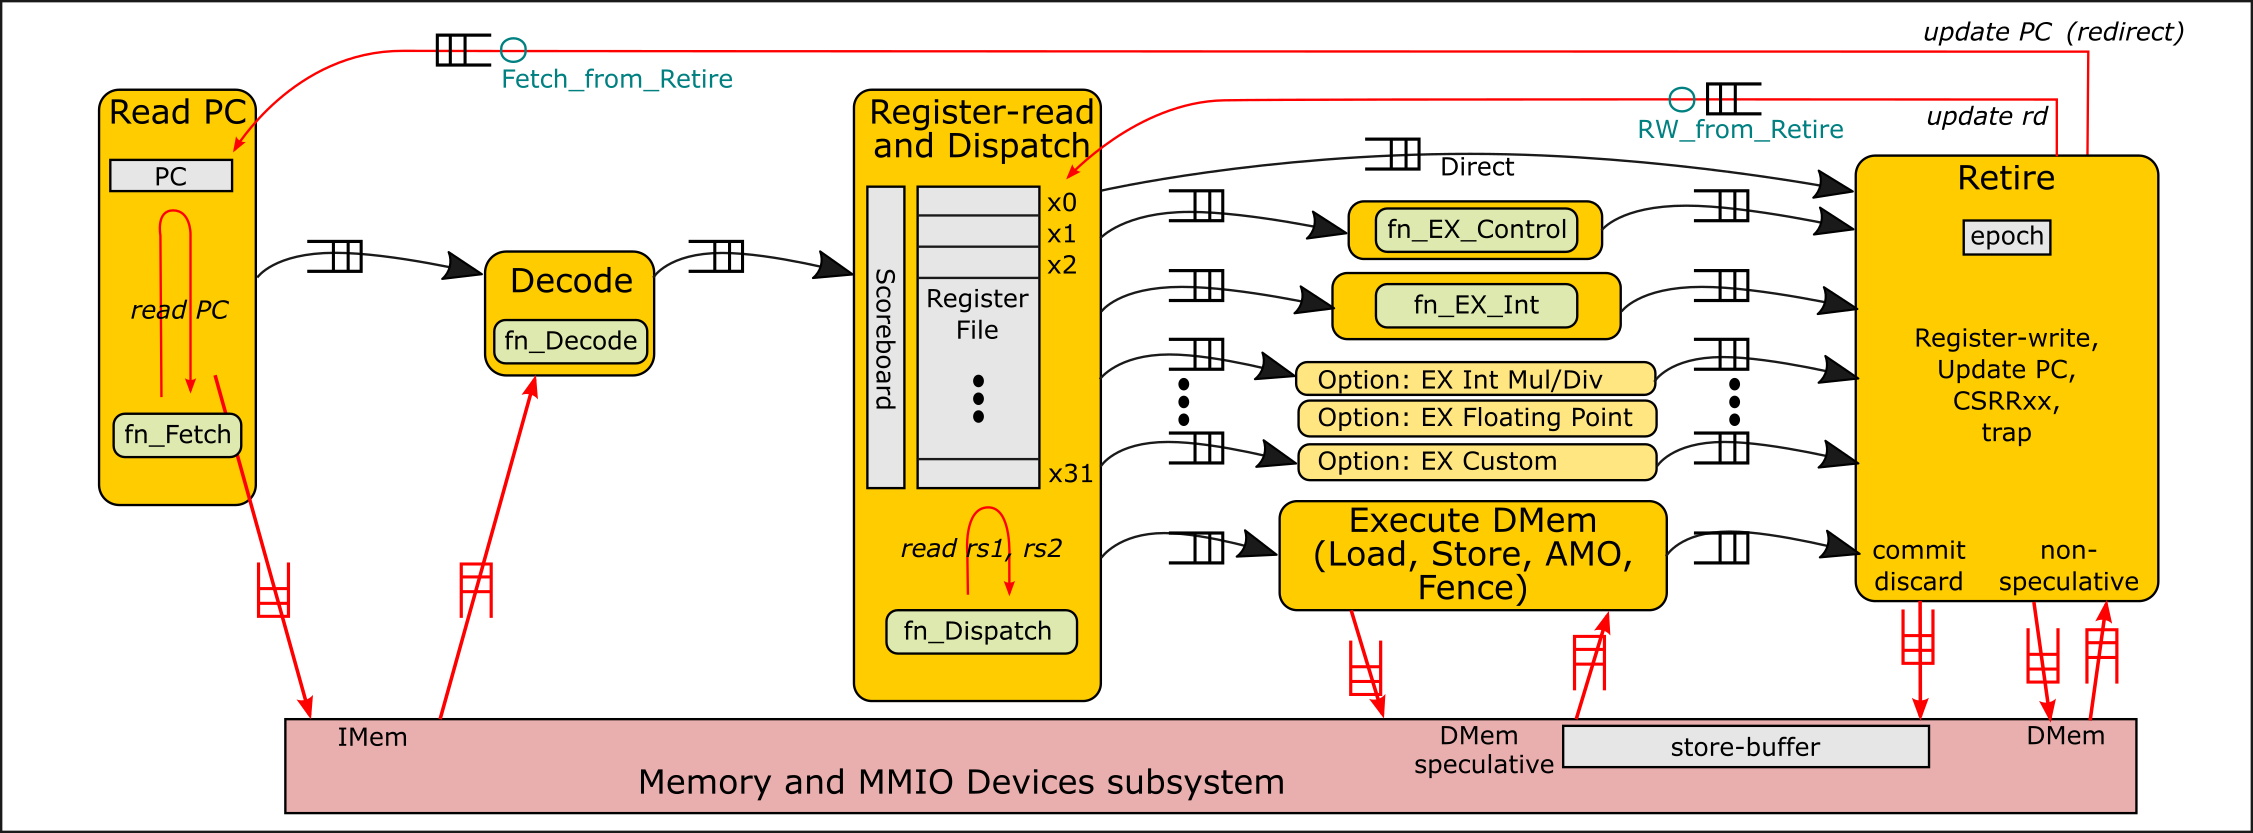
\includegraphics[width=6in]{Fig_Instr_Exec_w_FIFOs}}
  \centerline{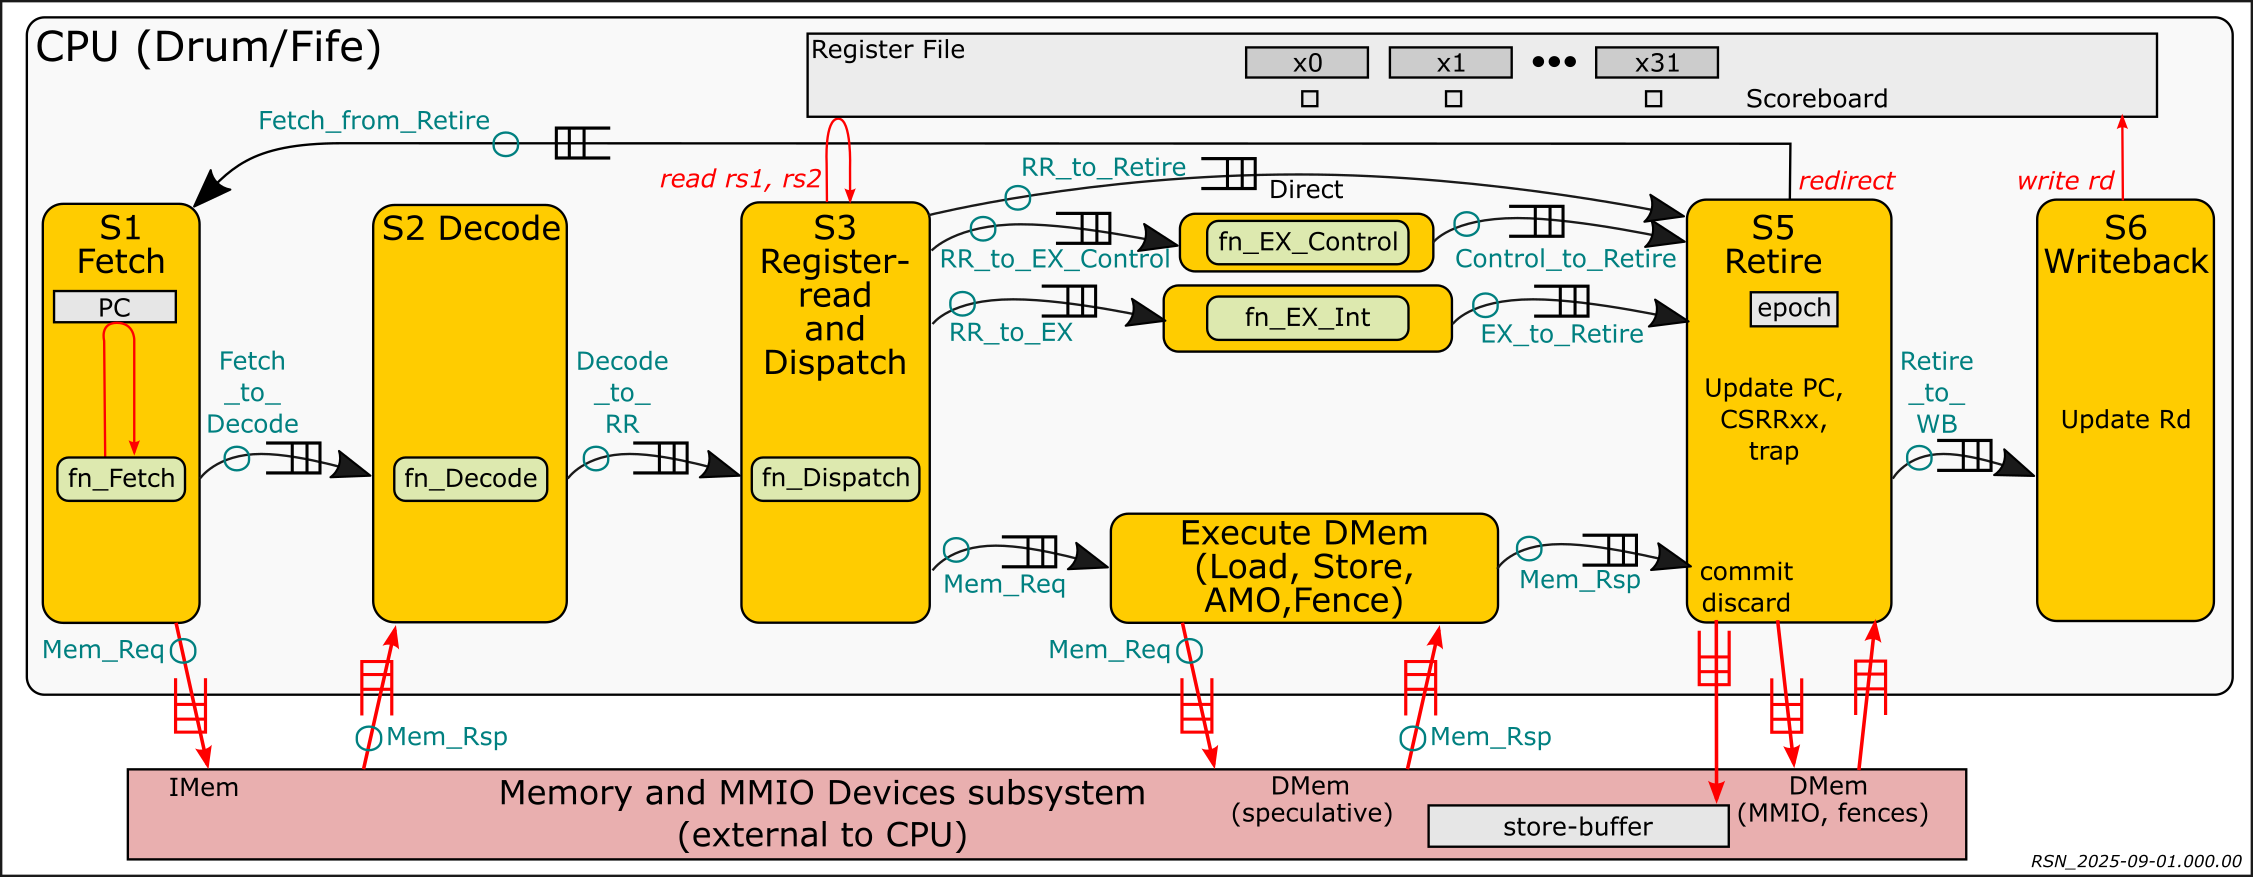
\includegraphics[width=6in]{RSN_2025-09-01.000.00_FifeDrum_Stages_Multilayer_L1_L2_L3}}
  \caption{\label{Fig_Instr_Exec_w_FIFOs}Pipelined interpretation of RISC-V instructions (Fig.~\ref{Fig_Instr_Exec} with some annotations)}
\end{figure}
Unlike Drum, where each yellow box was one step in a sequential
process, for Fife we interpret each yellow box as containing its own
infinite process.  There are now half-a-dozen or more processes in the
diagram (one for each yellow box), all running \emph{concurrently}.
Each black arrow in the diagram represents a flow of \emph{messages}
sent from one stage to another.  These messages are sent via FIFO
buffers (depicted by
\raisebox{-0.2ex}{\includegraphics[width=0.2in]{Fig_FIFO}}
annotations in the figure).

Each stage is an infinite loop, consuming incoming messages and
producing outgoing messages.  Thus, while the Retire stage is working
on instruction $n$, the Execute, Register-Read, Decode and Fetch
stage(s) may be working on instructions $n+1$, $n+2$, $n+3$, and
$n+4$, respectively.  Thus, there is a sequence, or train, of
instructions flowing through the diagram from left to right.

Pipelining raises four new problems, and these are the focus of this
chapter:

\begin{itemize}

  \item Continuing to Fetch, with PC Prediction and Epochs

  \item Managing Register Read/Write Hazards with a Scoreboard

  \item Retiring outputs of the Execute Stages in Order with Tags

  \item Allowing Memory Ops to be Pipelined with a Store Buffer

\end{itemize}

% ****************************************************************

\section{Continuing to Fetch, with PC Prediction and Epochs}

\label{Sec_Epochs}

What should the Fetch stage do after issuing a request to IMem for
instruction $n$?  To issue another request, it needs to know the PC of
instruction $n+1$, but there are several uncertainties about that next
PC:

\begin{tightlist}

 \item The current Fetch itself can raise an exception (trap) if its
        PC is misaligned, is an unsupported memory address, {\etc}.
        In this case the next PC will the trap-handler PC instead of
        the ``normal'' next PC.

 \item If it is a BRANCH instruction, until it reaches the Execute
       Control stage we do not know the branch target PC address, nor
       if the branch is taken or not.

 \item If it is a JAL or JALR instruction, until it reaches the
       Execute Control stage we do not know the target PC address.

 \item Many instructions can raise an exception (trap) (illegal
       instructions, BRANCH/JAL/JALR with misaligned target addresses,
       DMem ops with misaligned addresses or unsupported addresses,
       {\etc}); in these cases the next PC will the trap-handler PC
       instead of the ``normal'' next PC.

 \item The CPU may choose to respond to an external interrupt, in
        which case the next PC will be the interrupt-handler's
        address.

\end{tightlist}

Note, the Fetch stage knows nothing about instruction $n$ other than
its PC.  The instruction itself is not known until IMem sends its
response to the Decode stage (and assuming the Fetch does not raise an
exception).

% ================================================================

\subsection{PC Prediction in the Fetch Stage}

\index[RV]{Branch prediction}
\index[RV]{PC prediction}
\index[RV]{Prediction}
\index[RV]{Misprediction (wrong path instructions)}
\index[RV]{Wrong-path due (mispredicted instructions)}

A standard solution is for the Fetch stage to \emph{predict} the next
PC, {\ie} make a guess about the next PC.  Since all RISC-V RV32
instructions are 32-bits wide (4 bytes), and \emph{most} of them
``fall-through'' to the next adjacent instruction, a simple prediction
is: PC+4.  This prediction will be correct for most instructions, but
will be wrong for BRANCH instructions that take the branch, for
JAL/JALR instructions, and for any instruction that traps.  When the
prediction is wrong, the instructions that follow immediately are
called ``mispredicted'' or ``wrong-path'' instructions.

% ----------------
\vspace{2ex}

NOTE: \fbox{\small
\begin{minipage}{5in}

RISC-V instructions are all 32-bits wide, so PC+4 is a reasonably good
guess.  In ISAs that have variable-length instructions, prediction may
be more complicated.  Even in RISC-V, when implementing the ``C''
(Compressed Instructions) extension, some instructions may be 16-bits
wide, raising similar complications.

\vspace{1ex}

Earlier we said ``the Fetch stage knows nothing about instruction $n$
other than its PC''.  This is not strictly true--the CPU may have
fetched this PC before ({\eg} this PC is inside a loop, or in a
procedure that is called repeatedly).  Knowledge of past behavior can
improve the current prediction.  Most predictors in modern processors
use past history to improve and ``tune'' their branch predictors
dynamically while executing the program.  Designing good branch
predictors is a deep topic for which there are many good textbooks
(for example, \cite{Hennessy2017}).

\vspace{1ex}

PC prediction can be seen as a kind of ``machine learning''.  The
CPU's past execution history constitutes the ``training data'' for a
model, and the model is then asked to predict the next PC for the
current PC.

\end{minipage}}
% ----------------

% ================================================================

\subsection{Identifying and Flushing Wrong-path Instructions}

Clearly, we need to identify and flush wrong-path instructions from
the pipeline.  Figure~\ref{Fig_RISCV_Epochs} shows the general scheme.
\begin{figure}[htbp]
  \centerline{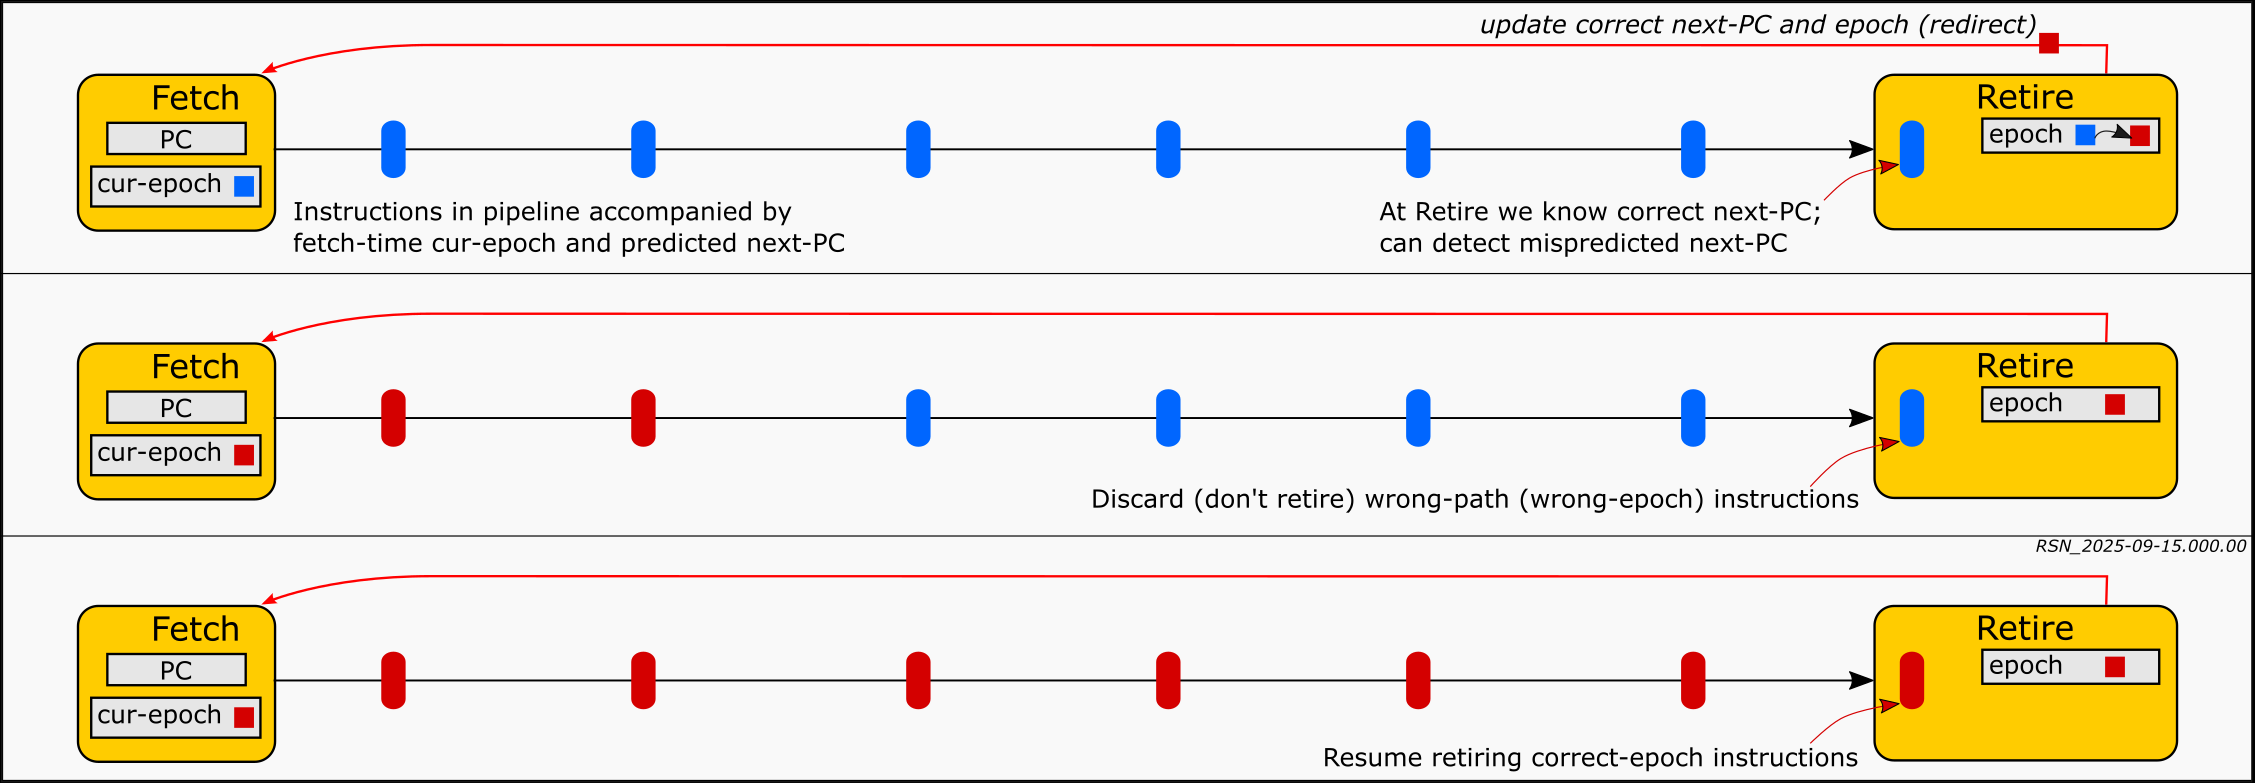
\includegraphics[width=\textwidth]{RSN_2025-09-15.000.00_Fife_Epochs}}
  \caption{\label{Fig_RISCV_Epochs}
           Using epochs to identify and discard mispredicted instructions}
\end{figure}

Suppose the Fetch stage issues requests for two instructions $i_1$ at
address $a_1$ and $i_2$ at address $a_2$, where $a_2$ is predicted
from $a_1$.  When issuing the request for $a_1$, the Fetch stage can
pass along $a_2$ to the Decode stage, from which point it can
accompany $i_1$ as it journeys through the pipeline ({\ie} every
instruction is accompanied by its next-PC prediction).

When $i_1$ reaches the Retire stage, we know the \emph{correct} next
PC (Trap handler PC?  PC+4?  Branch-taken target?  JAL/JALR target?).
By comparing this actual next PC with $a_2$, we know whether the
successor to $i_1$ was predicted correctly or not.

If we find that the prediction was correct, there is nothing more to
be done; we allow the pipeline flow to proceed.

\index[RV]{PC prediction!redirection}
\index[RV]{redirection on misprediction}

If we find that the prediction was wrong, then two things must happen:

\begin{itemize}

  \item We need to \emph{redirect} the Fetch stage to start fetching
    from the correct next-PC.  This involves sending a message from
    the Retire stage back to the Fetch stage containing the correct
    next-PC.  Suppose the first instruction fetched after this
    redirection is $j_1$.

  \item Instruction $i_2$, and possibly following instructions $i_3$,
    $i_4$, ... until $j_1$ are wrong-path instructions, and must be
    flushed.

\end{itemize}

\index[RV]{rg\_epoch@{\tt rg\_epoch} register for managing mispredictions}

When the Retire stage starts flushing wrong-path instructions $i_2$,
$i_3$, $i_4$, ... how does it know when it has reached the end of the
wrong-path sequence?  In other words, how does it know when it sees
$j_1$?  This is precisely the purpose of the \verb|rg_epoch| register
shown in Figure~\ref{Fig_Instr_Exec_w_FIFOs}.

Think of \verb|rg_epoch| as a counter that continuously counts upward.
Suppose the current value is $e_1$.  As described above, when the
Retire stage recognizes an instruction whose successor has been
mispredicted, we send a redirection message to the Fetch stage with
the corrected PC. The Retire stage also increments $e_1$ and sends the
incremented value as part of the redirection.  Each time the Fetch
stage is redirected, it remembers the new epoch value.  It also sends
this value down the pipeline, accompanying each instruction fetched
with this value.

Now, flushing wrong-path instructions in the Regire stage is easy:
$i_2$, $i_3$, $i_4$, ... will be accompanied by the old epoch value
$e_1$, whereas the first correct-path instruction $j_1$ will be
accompanied by the new epoch value $e_1+1$.  Thus, the Retire stage
knows exactly which instructions are wrong-path and it can discard
them.

% ----------------------------------------------------------------

\EXERCISE{Ex-15-A-Epoch-Bitwidth}

% ================================================================

\subsection{Terminology: Speculative Instructions and Commits}

\index[RV]{Commit the side-effects of an instruction}
\index[RV]{Speculative instruction}
\index[RV]{Speculation of instructions}

Before an instruction has reached the Retire stage, there is always
the possibility that an earlier instruction that is ahead of it in the
pipeline will branch/jump to a PC that was not predicted, or will
trap, making this instruction irrelevant.  Until this moment, we say
that the instruction is still ``\emph{speculative}''.  When it reaches
the Retire stage, we say that it's side-effects can be
``\emph{committed}''.

% ================================================================

\subsection{Speculative instructions should not have any side-effects}

It is not enough for the Retire stage just to discard mispredicted
instructions.  Instructions have side-effects: they may modify
registers and write to memory.  We must ensure that speculative
instructions make no modifications that are visible to right-path
instructions that follow, until they reach the Retire stage.  The
details of how this is accomplished will be seen in
Section~\ref{Sec_Store_Buffers} and Section~\ref{Sec_Fife_Retire_Principles}.

% ****************************************************************

\section{Managing Register Read/Write Hazards with a Scoreboard}

\label{Sec_Scoreboards}

\index[RV]{Scoreboard, to manage register read/write hazards}
\index[RV]{Hazards!Scoreboard for managing}

Suppose instruction $i_1$ writes to register $x_7$, and the following
instruction $i_2$ reads from register $x_7$.  Instruction $i_1$'s
write to $x_7$ only happens in the Retire stage.  If $i_2$ were to
follow behind $i_1$ immediately, it will be in the Exec stage, and
would have already read $x_7$ earlier when it was in the Register-Read
stage.  In other words, it would have read a \emph{stale} or obsolete
value $x_7$.  This is called a Read-Write \emph{hazard}, or a
read-after-write \emph{dependency}.

In this situation, we need to make $i_2$ wait in the Register-Read
stage until $i_1$ has completed its update of $x_7$.  This is
precisely the purpose of the \verb|scoreboard| shown in
Figure~\ref{Fig_Instr_Exec_w_FIFOs}.  The general scheme is shown in
Figure~\ref{Fig_RISCV_Scoreboard}.
\begin{figure}[htbp]
  \centerline{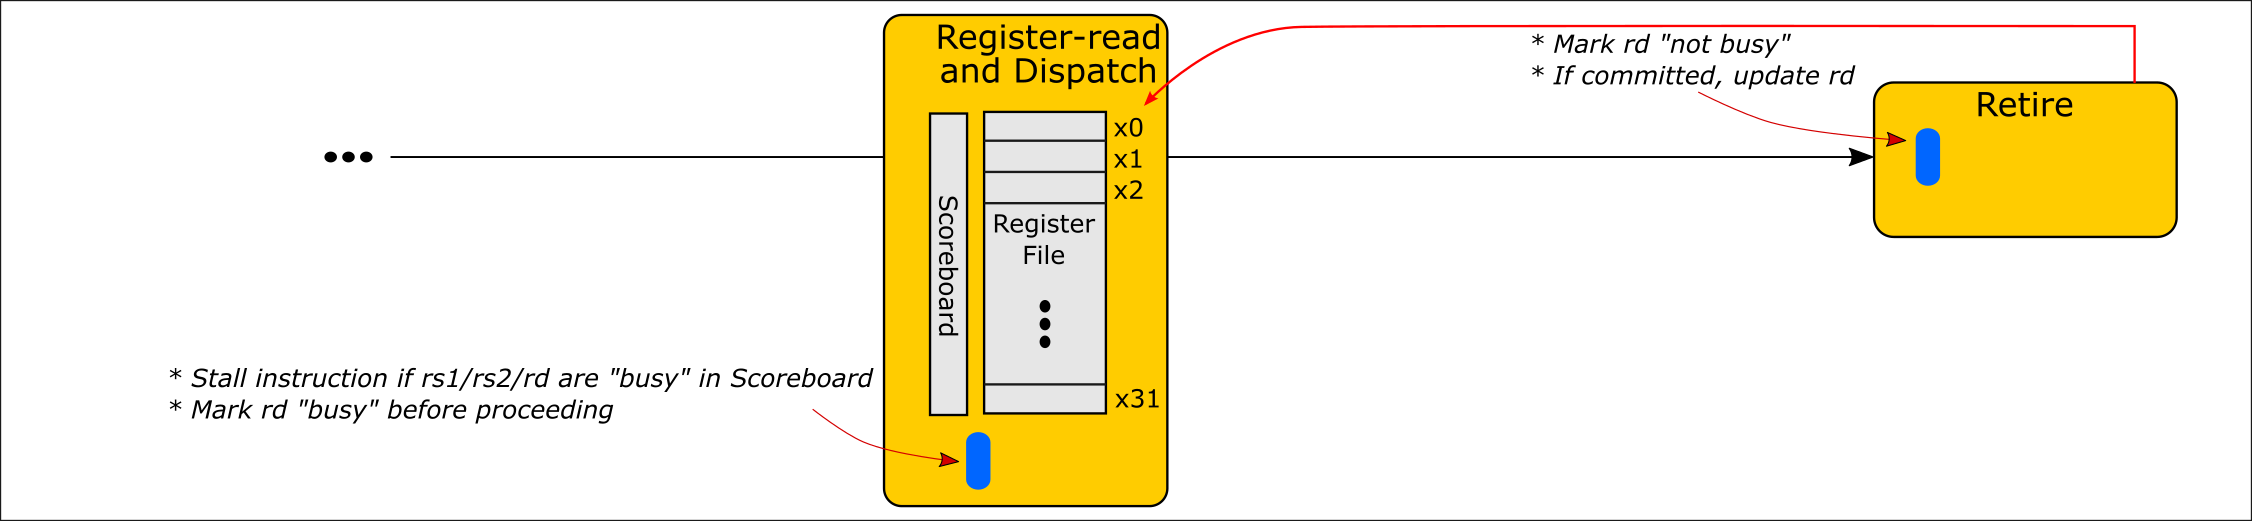
\includegraphics[width=\textwidth]{Fig_RISCV_Scoreboard}}
  \caption{\label{Fig_RISCV_Scoreboard}
           Using a scoreboard to manage register read/write hazards}
\end{figure}

The \verb|scoreboard| is an array of 32 1-bit registers (one bit for
each GPR).  When an instruction (such as $i_1$) passes through the
Register-Read stage, if it writes to register $x_7$, we set the
corresponding bit 7 in the scoreboard to 1, indicating that $x_7$ is
``busy''.  When $i_1$ reaches the Retire stage and writes to the
register, it also resets the scoreboard bit 7 to 0, indicating that
$x_7$ is ``not busy''.

When an instruction (such as $i_2$) reaches the Register-Read stage
and wants to read a register (such as $x_7$), if the corresponding
scoreboard bit says it is busy, then the Register-Read stage
``\emph{stalls}'', {\ie} it waits until the scoreboard condition is
cleared (by $i_1$ in the Retire stage).

\index[RV]{Pipeline!Bubble}
\index[RV]{Bubble in a pipeline}

While $i_2$ is waiting in the stalled Register-Read stage, note that
the following Execute stage may become ``empty'', {\ie} there is no
instruction occupying that stage.  We refer to this as a
``\emph{pipeline bubble}''.

% ----------------------------------------------------------------

\EXERCISE{Ex-15-B-Hazards}

\EXERCISE{Ex-15-C-Write-Write-Hazards}

\EXERCISE{Ex-15-D-Write-Write-ordering}

% ================================================================

\subsection{Releasing Scoreboard Reservations for Uncommitted Instructions}

When the Retire stage discards an instruction due to mis-speculation,
that instruction may be one which normally would have written a result
value into register $x_j$ in the register file.  If so, when it passed
through the Register-Read-and-Dispatch stage, it would have marked
register $x_j$ as ``busy'' in the scoreboard.  Now, when we discard
the instruction, even though we do not write any value into register
$x_j$, we still need to release the ``busy'' reservation on $x_j$
(otherwise, any succeeding instruction trying to read $x_j$ will get
stuck in the Register-Read stage.  Said another way, the reservation
in the scoreboard is a side-effect of this instruction that needs to
be rolled back.

% ================================================================

\subsection{Bypassing}

\label{Sec_Bypassing}

\index[RV]{Bypassing}
\index[RV]{Short-circuiting (bypassing)}

Digital hardware usually runs in time units of ``clock cycles''.  The
Retire stage writes a GPR (possibly) and writes the scoreboard (to
mark it ``not-busy'').  The Register-Read stage reads zero to two
GPRs, reads the scoreboard (to check ``not-busy'') and writes the
scoreboard (to set ``busy'').

\vspace{1ex}

For ordinary registers a write is only visible on the next clock
cycle.  Thus, if the scoreboard is just an ordinary register, the
Register-Read stage cannot observe ``not-busy'' until one clock after
the Retire stage has marked ``not-busy''.  This does not affect
correctness, but slows the performance of the CPU.

\vspace{1ex}

It is possible to design some extra circuitry around the scoreboard so
that the Register-Read stage can observe ``not-busy'' on the
\emph{same} clock cycle as when Retire marks it ``not-busy''.  This
technique is generically called ``\emph{bypassing}'' or
``\emph{short-circuiting}''.

% ----------------------------------------------------------------

\EXERCISE{Ex-15-E-Bypassing}

% ----------------------------------------------------------------

An even more advanced form of bypassing (with much more circuit
complexity) would be:

\begin{tightlist}

 \item Eliminate the scoreboard; do not stall an instruction in the
     Register-Read stage, but allow it to move into its appropriate
     Execute stage, and stall it there if necessary.  This frees up
     the Register-Read stage to process the next instruction, which
     may move into a different Execute stage.

 \item When Retire writes a register value, broadcast it to the
     different Execute stages to enable instructions there that are
     stalled on this register value.

\end{tightlist}

% ****************************************************************

\section{Retiring outputs of the Execute Stages in Order with Tags}

\label{Sec_Reorder_Tags}

\index[RV]{Tags!for proper instruction ordering}
\index[RV]{Tags!EXEC\_TAG\_DIRECT@{\tt EXEC\_TAG\_DIRECT}}
\index[RV]{Tags!EXEC\_TAG\_CONTROL@{\tt EXEC\_TAG\_CONTROL}}
\index[RV]{Tags!EXEC\_TAG\_IALU@{\tt EXEC\_TAG\_IALU}}
\index[RV]{Tags!EXEC\_TAG\_DMEM@{\tt EXEC\_TAG\_DMEM}}
\index[RV]{Instruction ordering!tags for}

As shown in Figure~\ref{Fig_RISCV_Retire_Ordering},
\begin{figure}[htbp]
  \centerline{\includegraphics[width=\textwidth]{Figures/Fig_RISCV_Retire_Ordering}}
  \caption{\label{Fig_RISCV_Retire_Ordering}
           Multiple pipelines in the Execute stage, of varying latencies}
\end{figure}
each yellow box in
the Execute stage is an independent pipeline handling a certain subset
of the instruction set.  For example, ``Execute Control'' handles
BRANCH, JAL and JALR instructions. ``Execute Integer Arithmetic and
Logic Ops'' handles LUI, AUIPC, and all arithmetic and logic
instructions.  ``Exec Mem Op'' handles LOAD and STORE instructions.
If we extend Fife to handle the ``M'' ISA extension, we would have a
pipeline for integer multiply and divide instructions.  If we extend
Fife to handle the ``F'' and ``D'' ISA extension, we would have a
pipeline for floating point arithmetic.  The
Register-Read-and-Dispatch stage sends information into these pipes
depending on the kind of instruction.

Instructions may have different latencies in traversing these Execute
pipes.  For example, Control and Integer ops may typically traverse in
one clock, but multiplication, division, floating point and memory ops
may take more clocks.  The latency variation may be data dependent:
for example multiplication/division may recognize the special case
where an operand is 0 or 1 and return a result quickly.  A memory op
may return quickly on a cache hit, and take more time on a cache miss.

The Retire stage needs to gather the outputs from the Execute stages
and retire them in the proper order.  But, because of varying latency,
availability of data is not an indication of the proper order.

The solution to this ``ordering'' problem is \emph{tags}.  In
Figure~\ref{Fig_Instr_Exec_w_FIFOs} we see there is also a
\emph{direct path} from Register-Read-and-Dispatch to Retire.  We pass
a tag on this path \emph{for every instruction}.  For example if the
instruction is a BRANCH instruction, the Register-Read-and-Dispatch
stage sends information into Execute Control, but it also sends a tag
\verb|EXEC_TAG_CONTROL| on the direct path to Retire, indicating that
it has just dispatched an instruction into Execute Control.

Thus, the sequence of tags on the direct path tells Retire exactly the
order in which to service the various Execute pipes.  Retire always
looks at tag on the direct path first.  For example, if Retire sees a
\verb|EXEC_TAG_DMEM| tag on the direct path, it knows that it must
next look for an output from the Exec Memory Ops pipe, even if outputs
are already available on the Execute Control and/or Execute Integer
pipes from later instructions.

% ****************************************************************

\section{Allowing Memory Ops to be Pipelined, with a Store Buffer}

\label{Sec_Store_Buffers}

\index[RV]{Store Buffer}

Consider the Execute Memory Ops stage in
Figure~\ref{Fig_RISCV_Store_Buffer},
\begin{figure}[htbp]
  \centerline{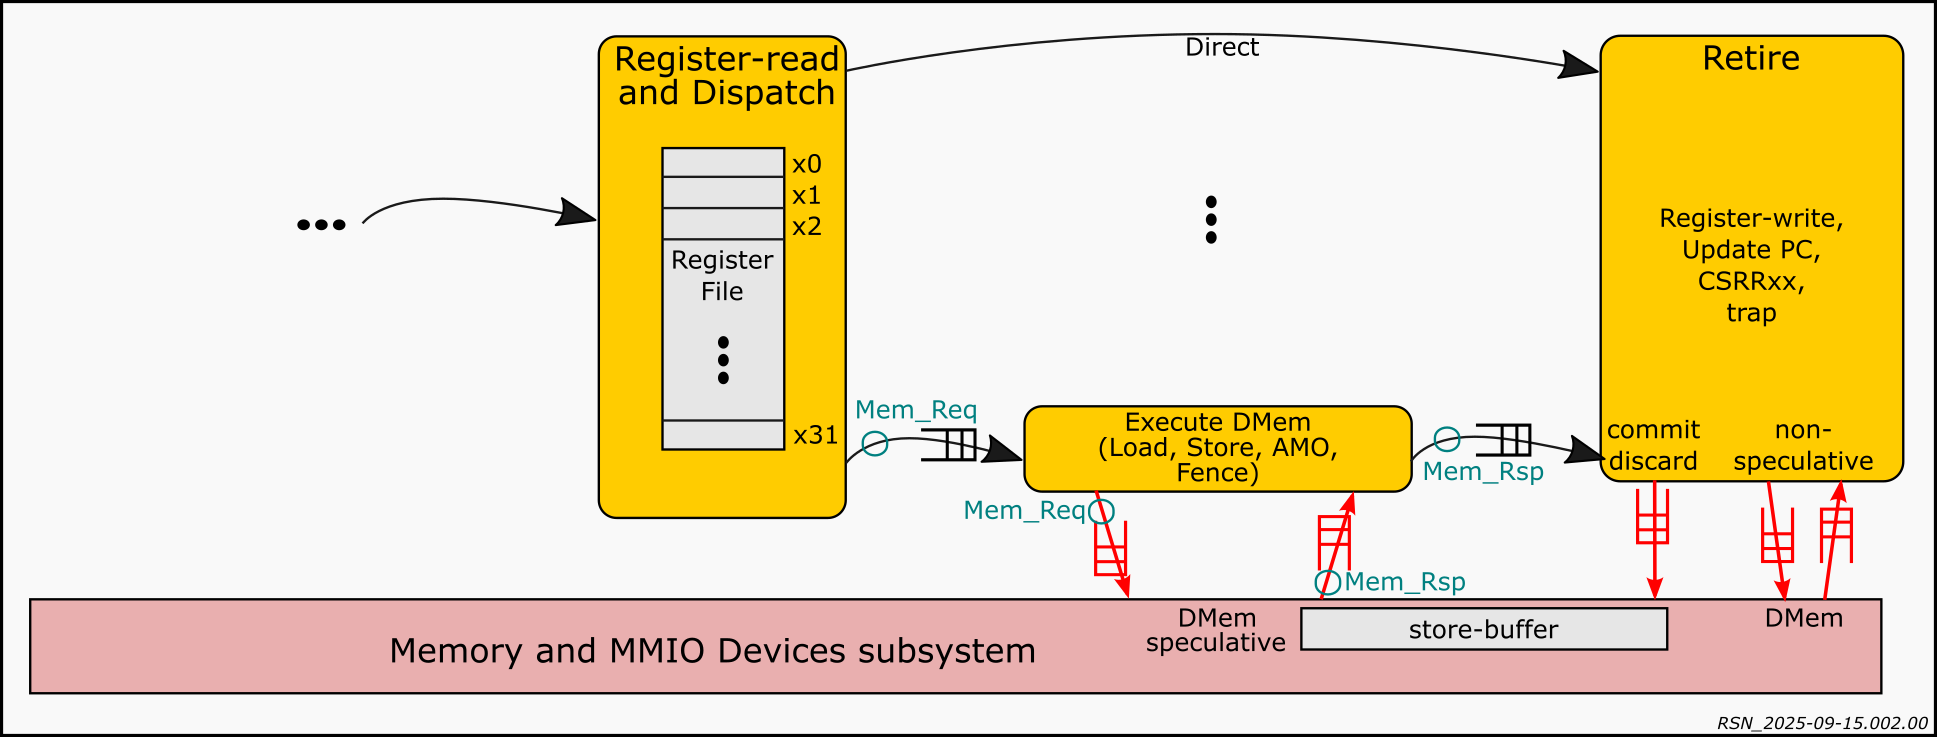
\includegraphics[width=\textwidth]{RSN_2025-09-15.002.00_Fife_Store_Buffer}}
  \caption{\label{Fig_RISCV_Store_Buffer}
           Speculative and non-speculative DMem access, with a Store Buffer}
\end{figure}
which issues LOAD and STORE requests to memory and collects their
responses.  At this stage, the instruction is still speculative; it
may be discarded when it reaches the Retire stage.  We must ensure
that STORE instructions do not yet modify memory permanently.

The mechanism for this purpose is the ``\emph{store buffer}'' shown in
the diagram.  This is a buffer in front of the memory system (between
the CPU and the memory system).

\begin{tightlist}

 \item The store buffer is itself a queue.

 \item When we execute a STORE instruction, the address, data and size
       are appended to the STORE buffer queue.  When the instruction
       finally reaches the Retire stage, the Retire stage sends a
       final ``commit/discard'' message to the store-buffer.  If a
       commit, the STORE at the head of the store-buffer is committed
       to memory and we dequeue it from the store-buffer.  If a
       discard, we just dequeue it from the store-buffer.

 \item When we execute a LOAD instruction, we first check the
       store-buffer if there have been any recent updates to the
       address in question, and then go to the memory system behind it
       if necessary.

\end{tightlist}

% ================================================================

\subsection{What about LOADs and STOREs to non-memory-like devices (MMIO)?}

\label{Sec_DMem_MMIO}

\index[RV]{MMIO (Memory-Mapped Input Output)}

In RISC-V there are no separate instructions for input and output to
devices.  Devices contain ``device registers'' which are placed at
particular ``memory addresses'' and are accessed from the CPU just
like memory, with LOAD and STORE instructions.  We say that the device
registers are ``mapped'' to those addresses.  These accesses can
control and configure the device, and move data between the CPU and
the device.  Such a scheme is known as MMIO, for Memory-Mapped
Input-Output.

Device registers, although addressed like memory locations, may behave
quite differently from memory, in several ways:

\begin{itemize}

  \item LOADs may have side-effects.  For example, a LOAD from a
    memory location does not (observably) disturb anything, but a LOAD
    from a device could switch on an LED, or increment a counter.

  \item LOADs may not be idempotent (two identical LOADs cannot be
    coalesced into one).  For example, two successive LOADs from a
    memory location return the same value, whereas two successive
    LOADs from, say, a UART's ``receiver buffer register'' may return
    two successive (and different) characters from a keyboard.

  \item STOREs may have additional side-effects.  A STORE to a memory
    location merely stores the value there.  A STORE to a device
    register may display it on a screen, start a motor, release a
    wheel brake, and so on.

  \item STOREs may not be idempotent (two identical STOREs cannot be
    coalesced into one), because each may have its own side-effect.

  \item In memory, a LOAD returns the value stored there by the most
    recent STORE.  For a UART device, on the other hand, a STORE may
    display a character on a screen whereas a subsequent LOAD from the
    same address may return a character from the keyboard.

\end{itemize}

For these reasons, it is dangerous to perform any LOAD or STORE
speculatively on non-memory devices.  The ``Execute Memory Ops'' stage
does not even attempt the access; it simply defers such a request for
future execution by the Retire stage.  The decision whether to defer a
request or not is based on the address.

Once the LOAD/STORE instruction has reached the Retire stage and we
know for sure that it is not speculative, the Retire stage performs
the memory operation: it sends the request to memory, collects the
response, and retires the instruction.


% ----------------------------------------------------------------

\EXERCISE{Ex-15-F-Store-Buffers}

% ****************************************************************

\section{The Retire Stage}

\label{Sec_Fife_Retire_Principles}

Figure~\ref{Fig_Fife_Retire} summarizes the actions to be taken by
Fife's Retire stage.

\begin{figure}[htbp]
  \centerline{\includegraphics[width=6in,angle=0]{Fig_Retire_Layers_1_2}}
  \caption{\label{Fig_Fife_Retire}Retire actions in Fife}
\end{figure}

Much of this is the same as in Figure~\ref{Fig_Retire_Drum} for Drum.
The new additional details are:

\begin{itemize}

 \item The ``update PC'' operation now sends a message to redirect
       Fetch \emph{only} if the successor to the current PC had been
       mispredicted.  Recall that we carry the predicted PC value
       along with the instruction through the pipe, so here we can
       compare the now-known actual next PC with the predicted PC.

       If we redirect, we increment the \verb|epoch| number and send
       the new epoch number along with the redirection.  Any
       subsequent instructions with the old epoch number are ``wrong
       path'' instructions and must be discarded.

 \item Wrong path: any of the Execute pipes can produce a wrong-path
       instruction (accompanying epoch does not match current epoch).
       In each such case, we discard the instruction, but there are two more needed actions:

       \begin{tightlist}

        \item If the instruction has an \verb|Rd|, we would have taken
              a scoreboard reservation for it in the Register-Read
              stage; we must now release that scoreboard reservation.
              We extend \verb|update_rd| to perform a
              scoreboard-release without a register-write.

        \item In the case of a non-deferred STORE instruction, we
              would have placed an entry in the store-buffer.  We use
              ``finalize store buffer'' to discard that entry.

       \end{tightlist}

 \item Correct path non-deferred STORE instruction: we would have
        placed an entry in the store-buffer.  We use ``finalize store
        buffer'' to commit that entry to memory.

 \item ``Deferred'' memory request from DMem (because it was for an
       non-memory-like address such as MMIO): If so, the second Exec
       Mem Ops box in the figure now performs the DMem operation.

\end{itemize}

% ****************************************************************
